\begin{columns}[totalwidth=.85\linewidth]
	\column{\textwidth}
	\vspace{-10mm}
		\begin{itembox}[l]{Strand Length (N = 36) and Shear Stress for 4-Chains}
			\begin{itemize}
				\item System
				\begin{itemize}
					\item Strand length N = 36
					\item Multiplicity = 3
				\end{itemize}
				\item Deformation
				\begin{itemize}
					\item Shear mode (Lees-Edwards)
					\item Shear rate = $1e^{-5}$
				\end{itemize}
			\end{itemize}

			\begin{figure}[htb]
				\centering
					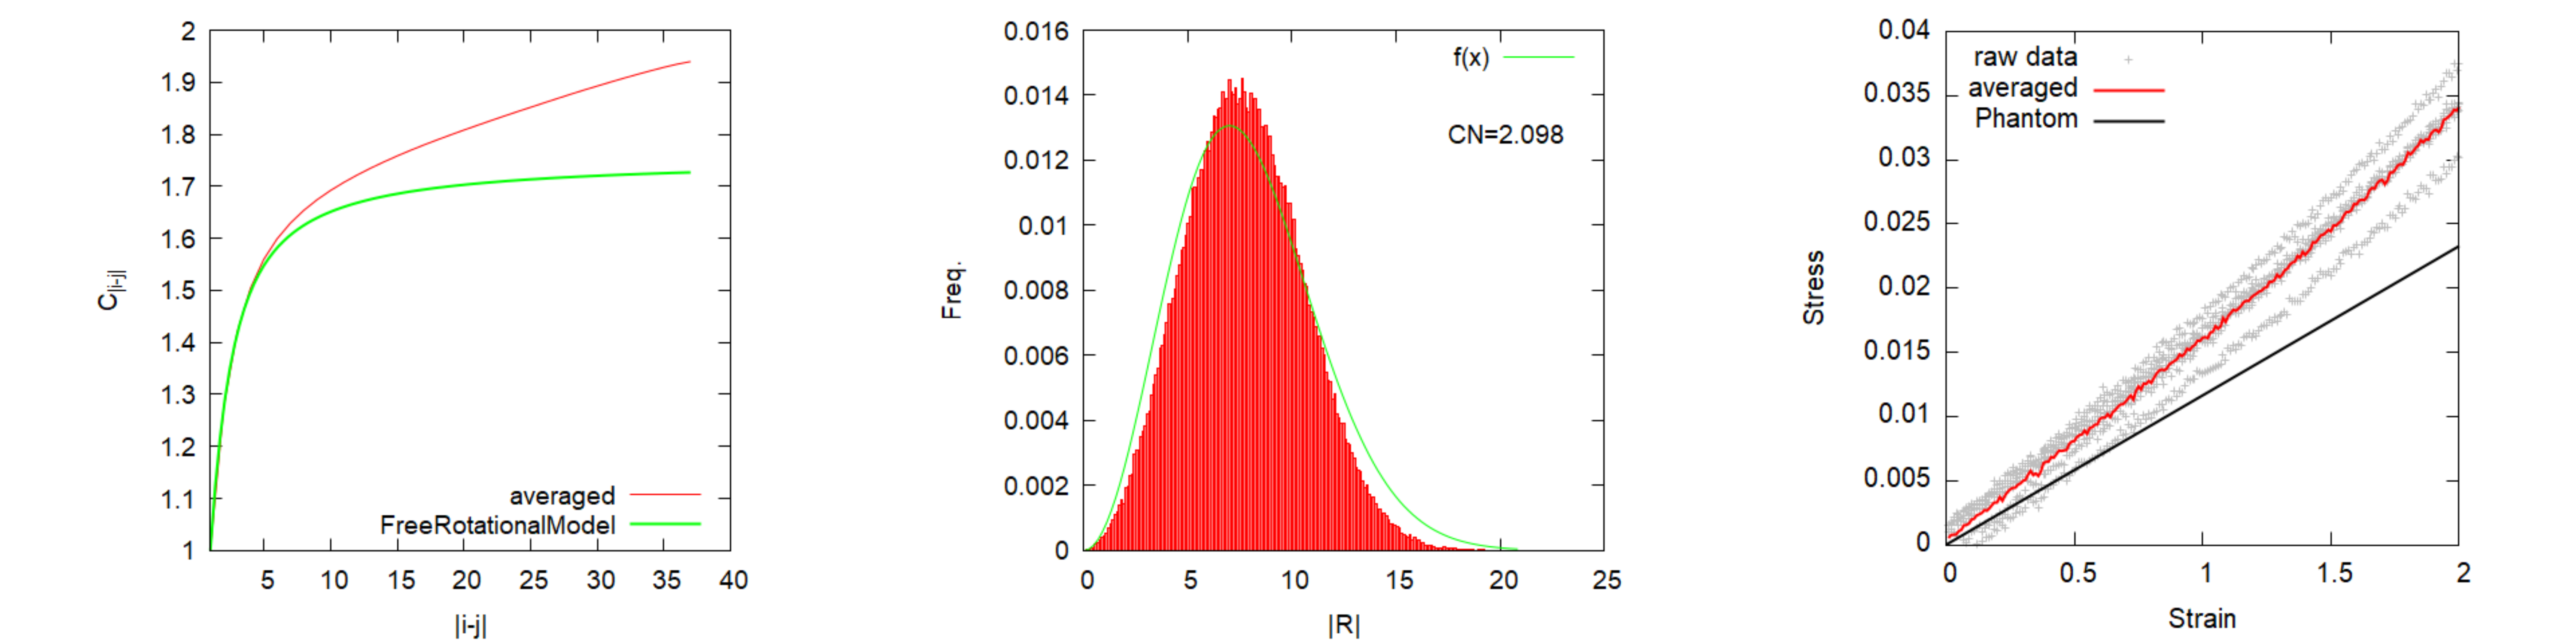
\includegraphics[width=.8\textwidth]{N36_result.png}
					\caption{Simulation results for 4-Chain model:N = 36, M = 3}
					\label{4_N36}
			\end{figure}
		\end{itembox}

		\begin{itembox}[l]{Strand length Effect for 4-Chains}
			\begin{itemize}
				\item Strand length is varied from 36 to 48
				\item System size is reduced to keep $\rho = 0.85$
			\end{itemize}

			\begin{figure}[htb]
				\centering
					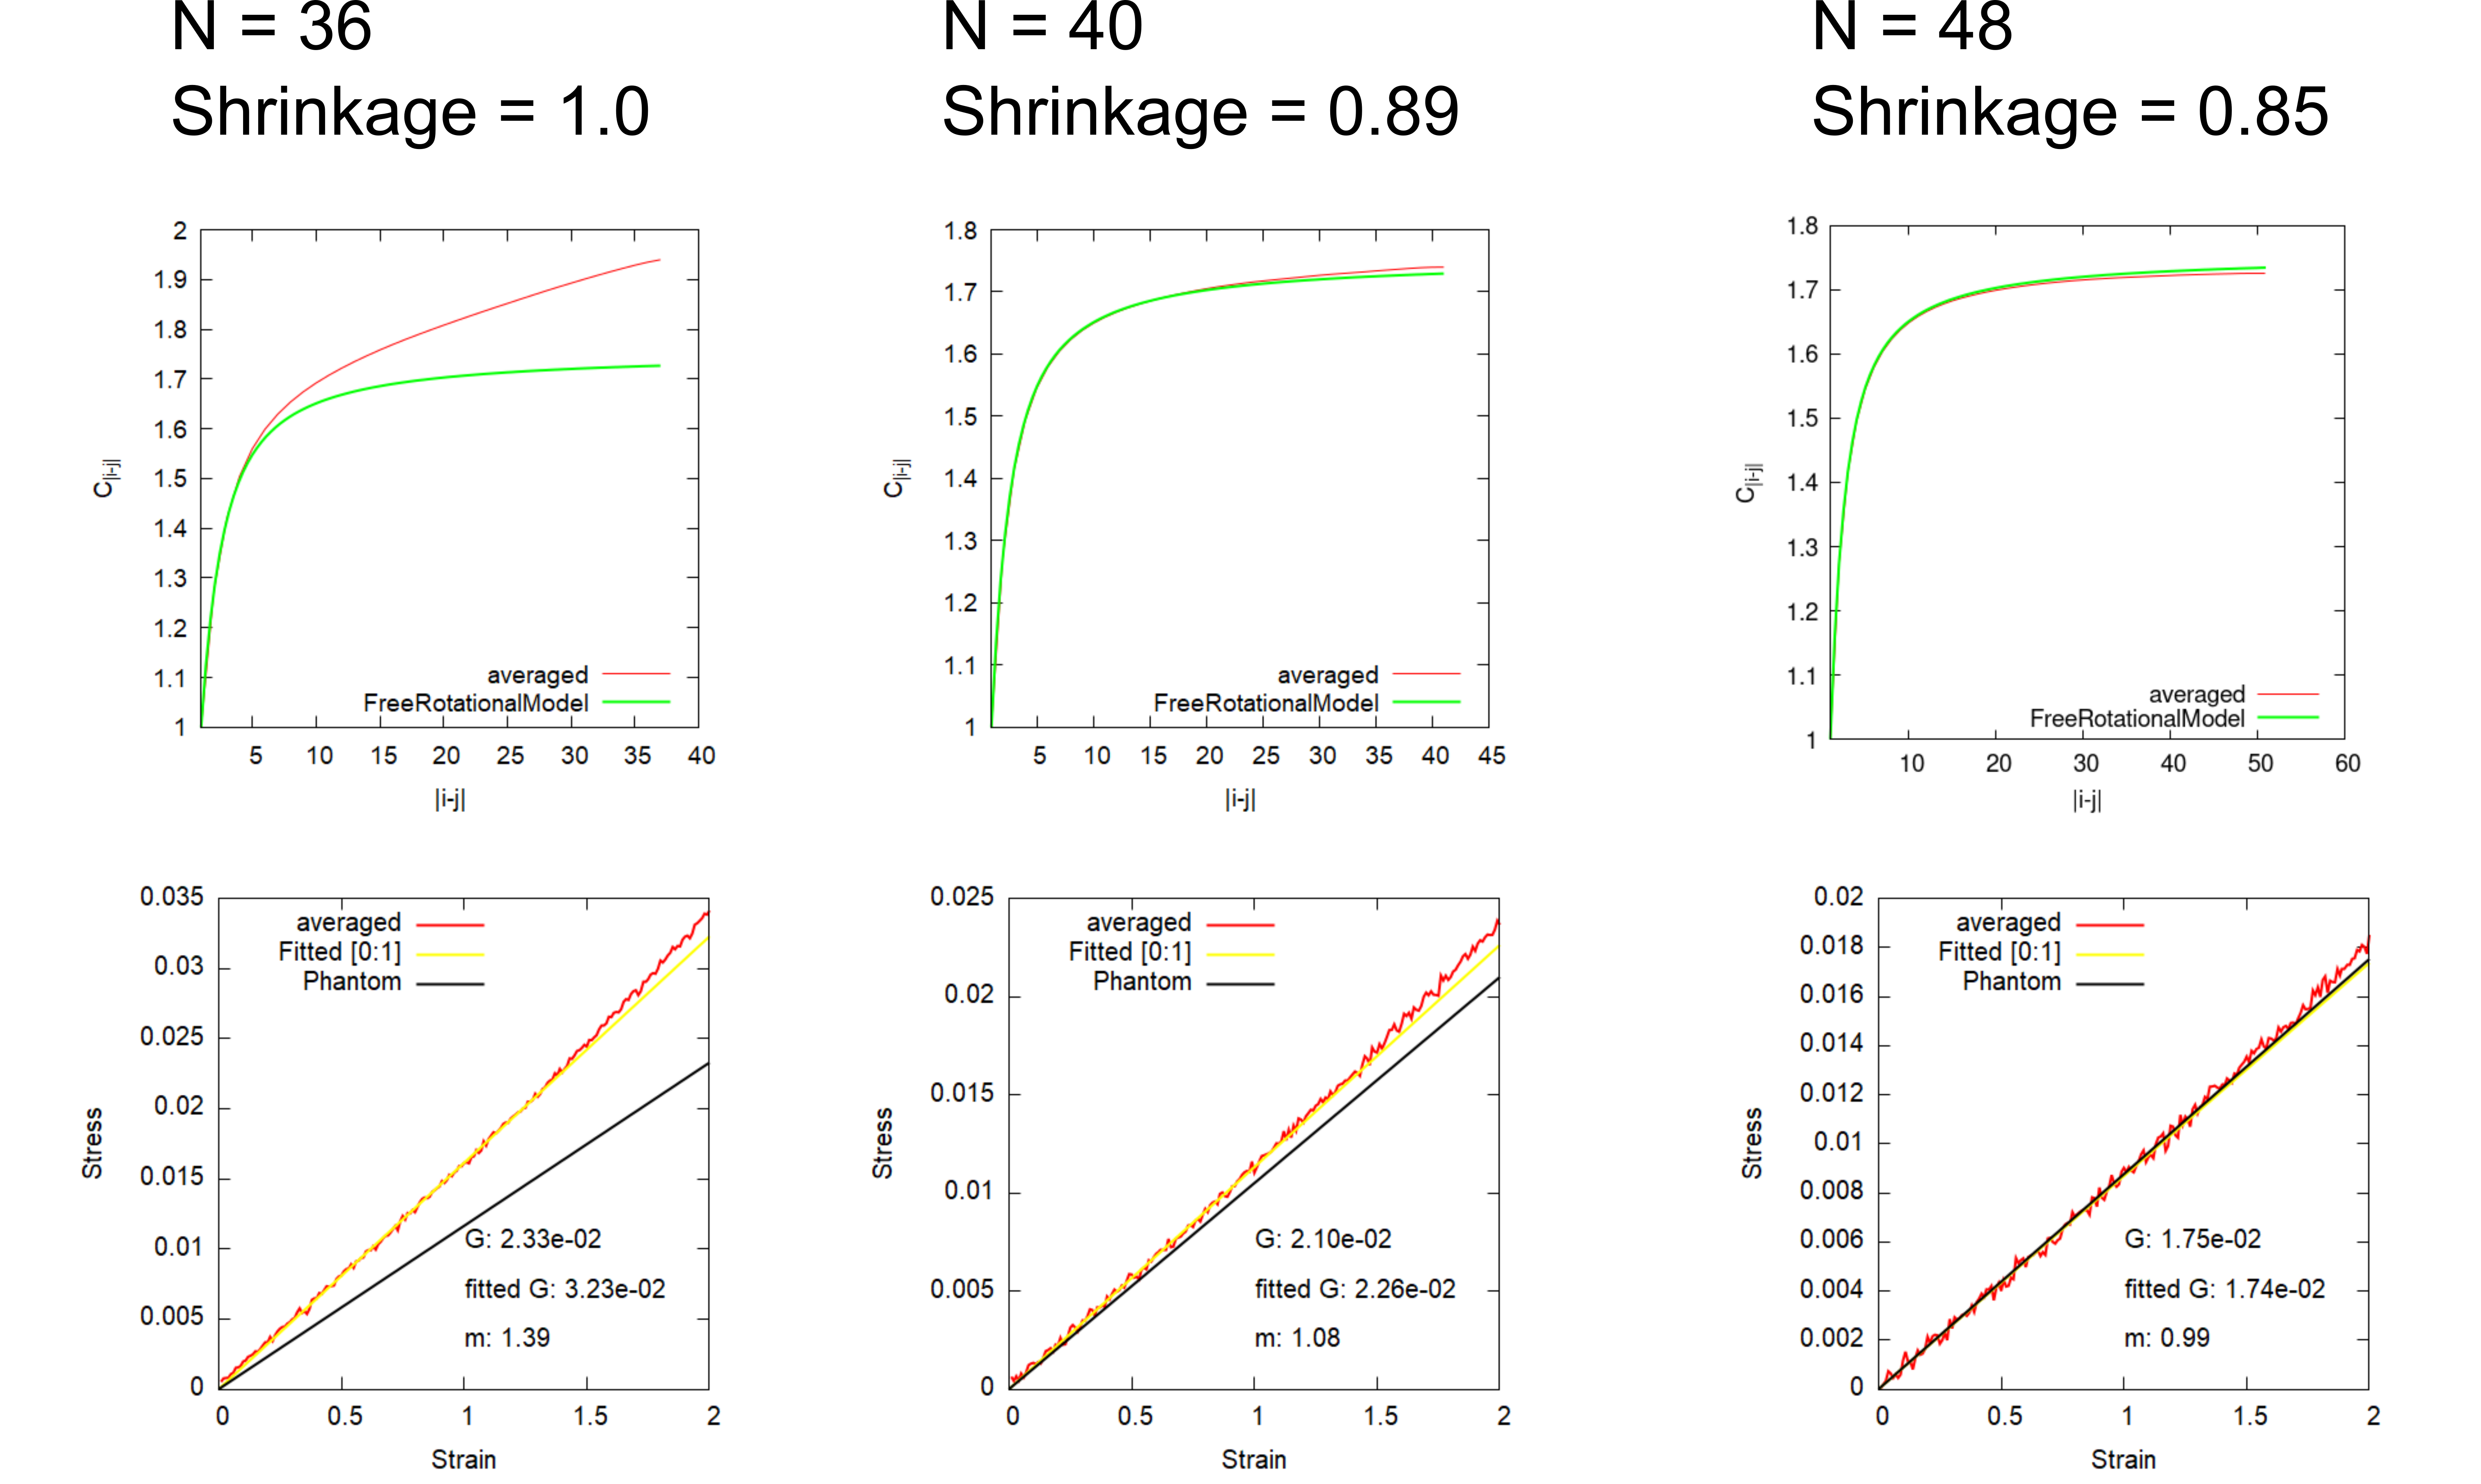
\includegraphics[width=.8\textwidth]{N36_N40_N48.png}
					\caption{Strand Length Comparison for N = 36, 40, 48}
					\label{4_N364048}
			\end{figure}
		\end{itembox}

		\begin{itembox}[l]{Comparison of Functionality (f = 3, 4, 6)}
			\begin{itemize}
				\item Using same length of strand (N = 48), functionality effect was compared.
			\end{itemize}

			\begin{figure}[htb]
				\centering
					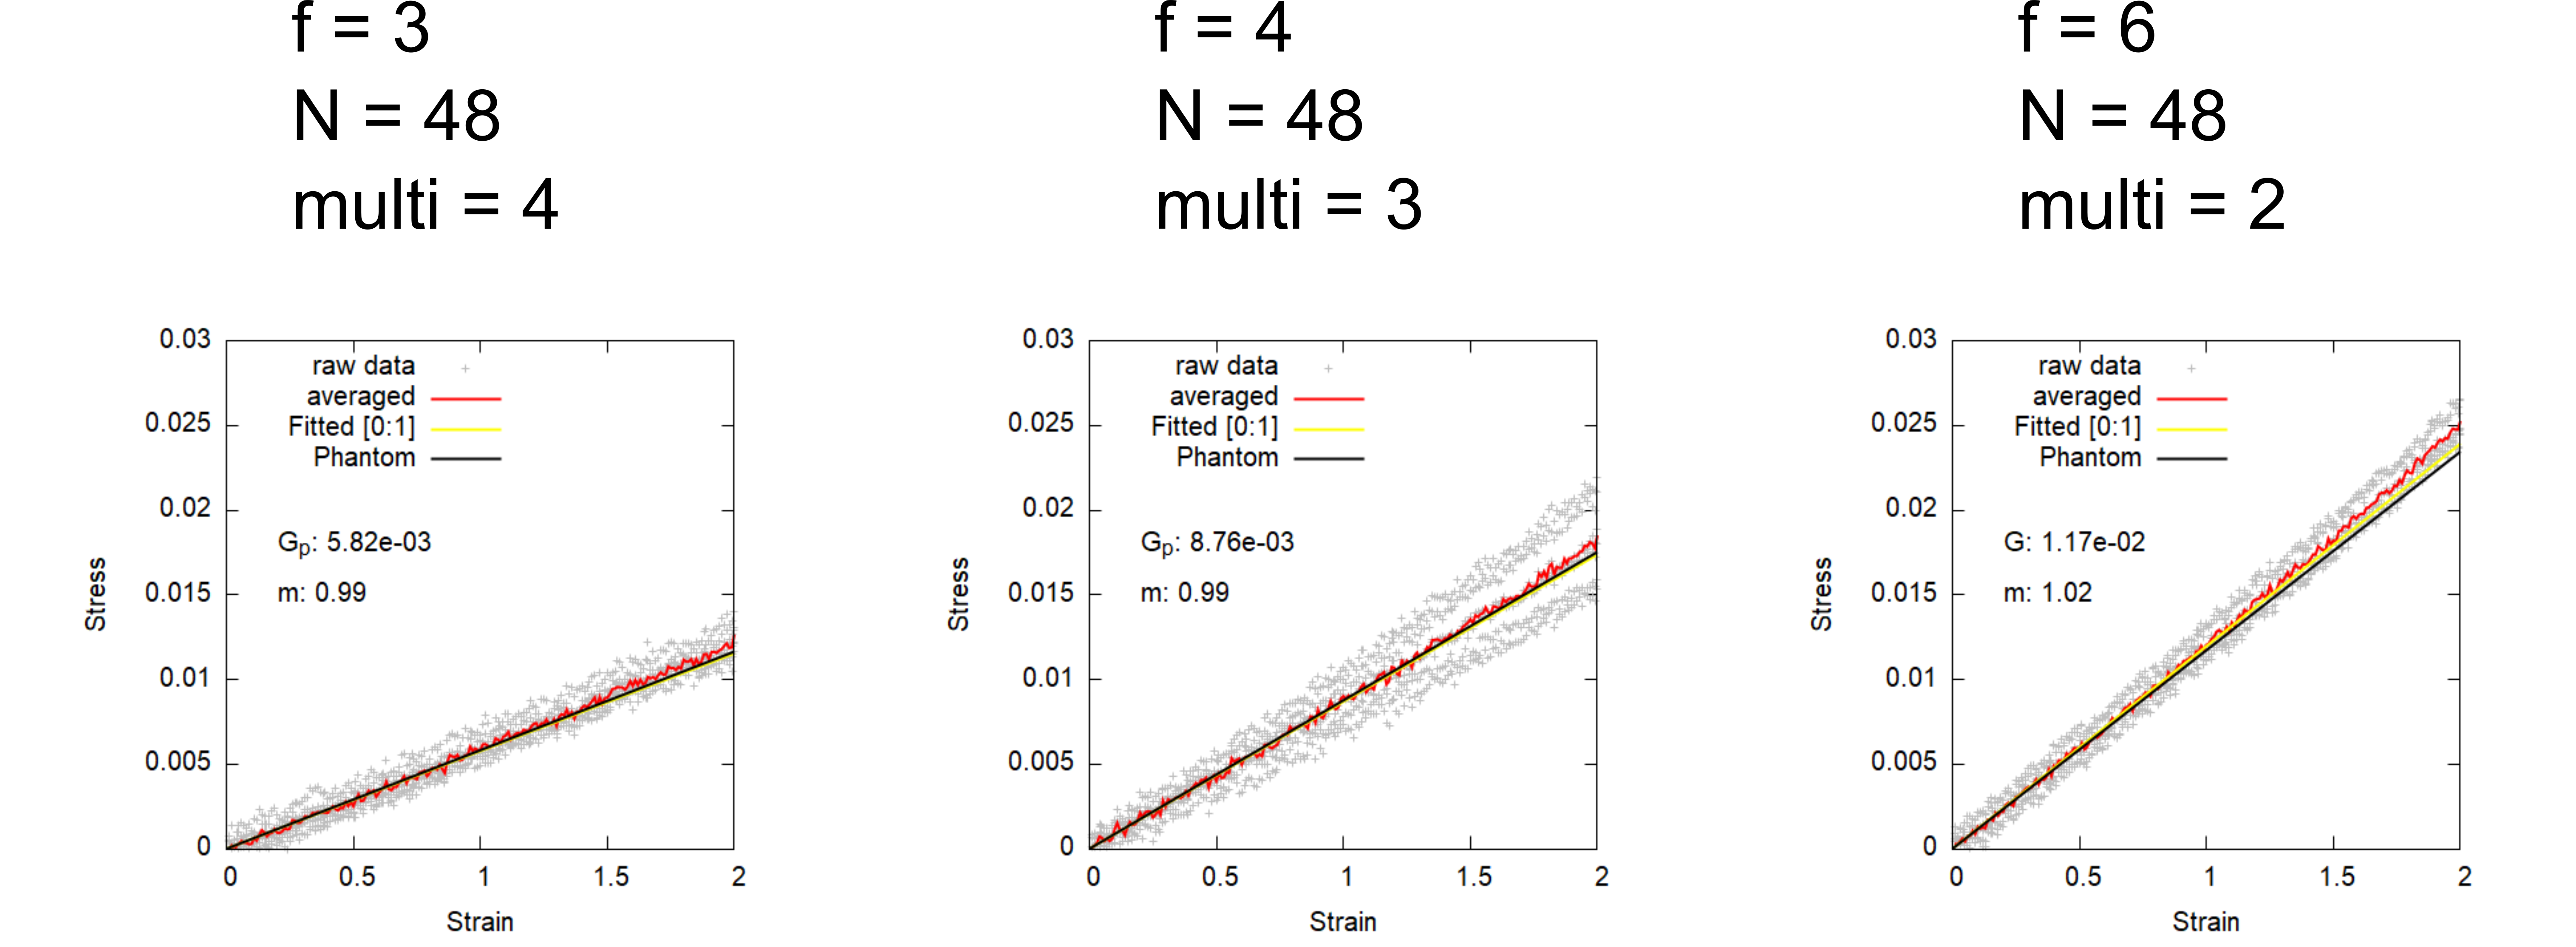
\includegraphics[width=.8\textwidth]{compare_346.png}
					\caption{Comparison of Functionality (f = 3, 4, 6)}
					\label{N48_f346}
			\end{figure}
		\end{itembox}
\end{columns}